\section{J-PARC E31 experiment and $d(K^-, n)$ reaction}

\begin{figure}
  \begin{tabular}{cc}
    \begin{minipage}{0.5\hsize}
      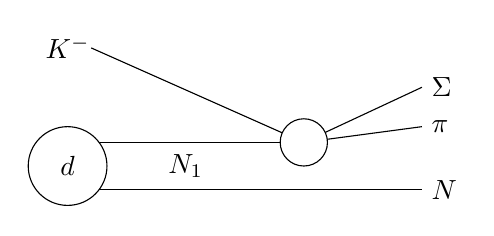
\begin{tikzpicture}
        \draw (0.0, 1.5) node {$K^-$};
        \draw (0.3, 1.5)-- (3, 0.3);      
        \draw (0,  0.3) -- (3,  0.3);
        \draw (0, -0.3) -- (4.5, -0.3) [right] node{$N$};
        \draw (3,  0.3) -- (4.5, 0.5) [right] node{$\pi$};
        \draw (3,  0.3) -- (4.5, 1.0) [right] node{$\Sigma$};
        
        \draw [fill=white](3, 0.3) circle (0.3);
        \draw [fill=white](0, 0) circle (0.5) node{$d$};

        \draw node at (1.5, 0.0){$N_1$};
      \end{tikzpicture}
    \end{minipage}
    
    \begin{minipage}{0.5\hsize}
      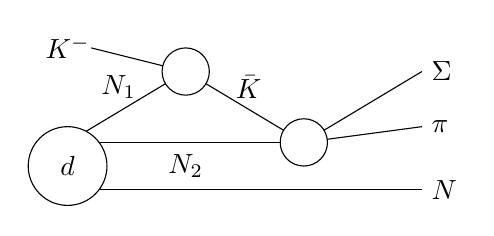
\begin{tikzpicture}
        \draw (0.0, 1.5) node {$K^-$};
        \draw (0.3, 1.5)-- (1.5, 1.2);
        \draw (0,  0.3) -- (3,  0.3);
        \draw (0, -0.3) -- (4.5, -0.3) [right] node{$N$};
        \draw (3,  0.3) -- (4.5, 0.5) [right] node{$\pi$};
        \draw (3,  0.3) -- (4.5, 1.2) [right] node{$\Sigma$};

        \draw (1.5, 1.2)-- (3.0, 0.3);
        \draw (0.0, 0.3)-- (1.5, 1.2);      
        \draw [fill=white](1.5, 1.2) circle (0.3);
        \draw [fill=white](3.0, 0.3) circle (0.3);
        \draw [fill=white](0, 0) circle (0.5) node{$d$};

        \draw node at (2.3, 1.0){$\bar{K}$};
        \draw node at (0.65, 1.0){$N_1$};
        \draw node at (1.5, 0.0){$N_2$};
      \end{tikzpicture}
    \end{minipage}
  \end{tabular}
  \caption{
    Fynman diagrams about $d(K^-, N)"\pi\Sigma"$ reaction.
    The left and right figures indicate about 1-step and 2-step reactions, respectively.
  }
  \label{fig:kd_diag}
\end{figure}

%% \begin{figure}[htbp]
  \centering
  \includegraphics[width=10cm]{pic/intro/Jido_Braun.png}
  \caption{
    This figure shows $\pi^+ \Sigma^-$ spectra of $K^- + d \rightarrow \pi^+ + \Sigma^- + n$ with 800 MeV incidnet $K^-$ momentum calculated by the chiral unitary model\cite{Jido2} (solid line) and
    experimental data measured by the bubble chamber \cite{Braun} (error bar).
  }
  \label{fig:Jido_Braun}
\end{figure}

%% \begin{figure}[htbp]
  \centering
  \includegraphics[width=12cm]{pic/intro/AGS_E31.png}
  \caption{
    $K^-d \rightarrow n \pi \Sigma$ calculated spectra using AGS equation by Ohnishi et el.\cite{Ohnishi}.
    Left and right figures indicate energy independent and dependent model, respectively.
    $\pi^+ \Sigma^-$, $\pi^0\Sigma^0$ and $\pi^-\Sigma^+$ indecate red solid line, blue dotted line and green dash line.
  }
  \label{fig:AGS_E31}
\end{figure}

%% \begin{figure}[htbp]
  \centering
  \includegraphics[width=12cm]{pic/intro/Miyagawa.png}
  \caption{
    Theoretical calculation using Faddev eqation by Miyagawa et el.\cite{Miyagawa}.
    Left top, right top, left bottom and right bottom figures represent about $\pi^-\Sigma^+$, $\pi^+\Sigma^-$, $\pi^-\Sigma^0$ and $\pi^0\Sigma^0$ channel, respectively.
    The result of $\pi^-\Sigma^+$, $\pi^+\Sigma^-$ and $\pi^-\Sigma^0$ by pilot run of J-PARC E31 experiment \cite{E31_pilot} is plotted at same figure.
    Red, green and blue indicates recent analysis by A. Cieplý and J. Smejkal \cite{WT1},
    energy dependent model by Ohnishi et el. \cite{Ohnishi} and old analyssi by E. Oset, A. Ramos, and C. Bennhold \cite{ORB}.
    Red dash vertical lines indicates $K^0 n$ (higher) and $K^-p$ (lower) mass threshod.
  }
  \label{fig:Miyagawa}
\end{figure}

%% \begin{figure}[htbp]
  \begin{tabular}{ccc}
    \begin{minipage}{0.33\hsize}
      \centering
      \dKNpimSp\\
      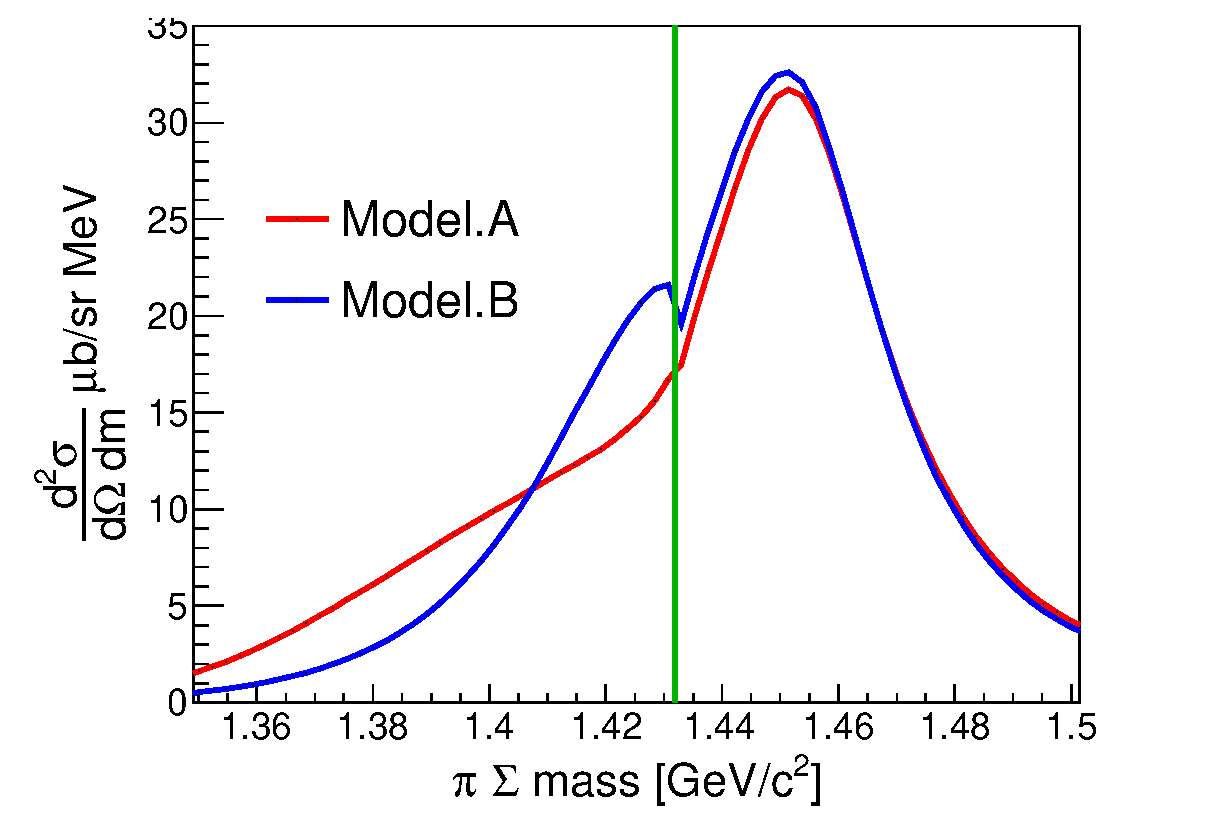
\includegraphics[width=4.3cm]{../pic/discussion/DCC_pimSp.eps}
    \end{minipage}

    \begin{minipage}{0.33\hsize}
      \centering
      \dKNpipSm\\
      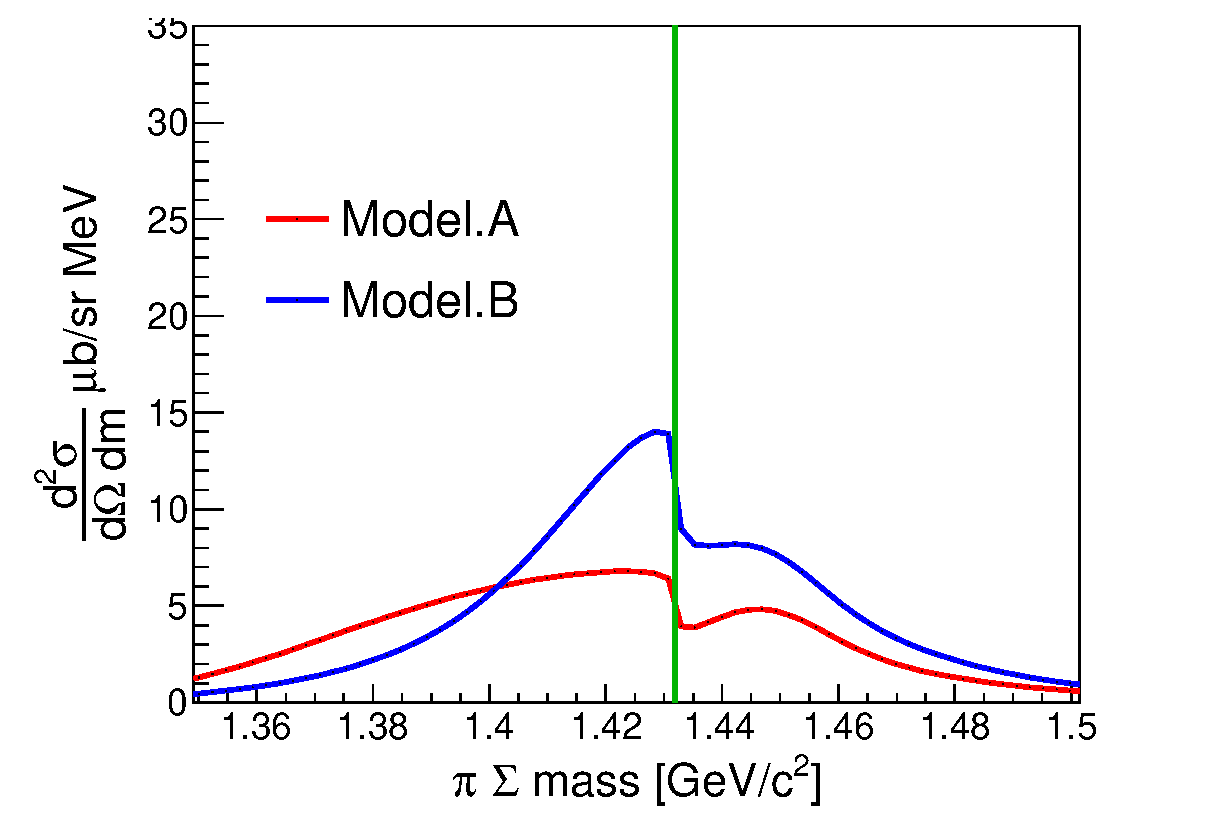
\includegraphics[width=4.3cm]{../pic/discussion/DCC_pipSm.eps}
    \end{minipage}

    \begin{minipage}{0.33\hsize}
      \centering
      \dKPpimSz\\
      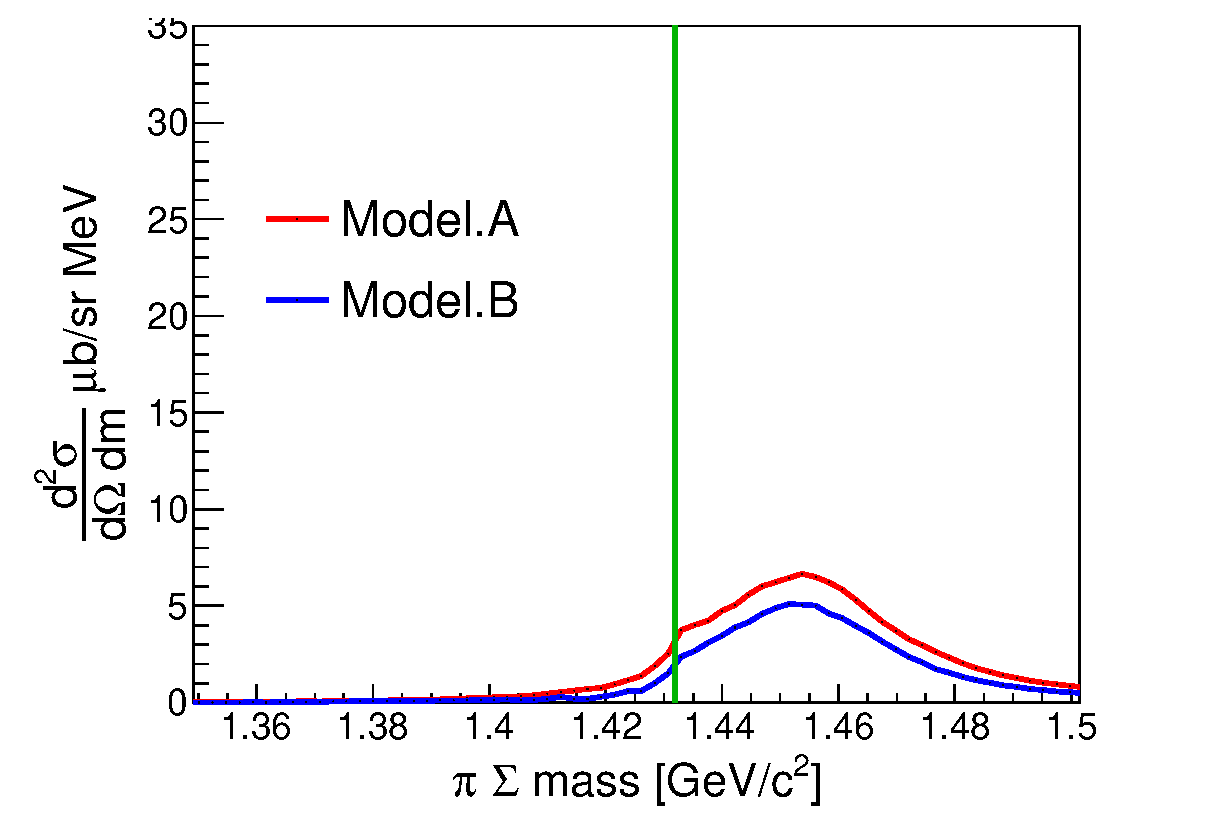
\includegraphics[width=4.3cm]{../pic/discussion/DCC_pimS0.eps}
    \end{minipage}
  \end{tabular}
  \caption{
    The calculated spectra by the DCC method \cite{DCC2}.
    Left, center and right figures show \pimSp, \pipSm and \pimSz, respectively.
    Red and blue lines represent model.A and B, respectively.
    Green vertical line indicates the $K^-p$ mass threshold.
  }
  \label{fig:DCC_kd}
\end{figure}
 
In this situation, direct measurement of $\bar{K}N\rightarrow \pi\Sigma$ scattering is desired. 
But the reaction can not happen in free space due to energy conservation.

This reaction using a $K^-$ beam of $644$-$844$MeV$/c$ has been measured at CERN using a bubble chamber and a $K^- d \rightarrow n \pi^+\Sigma^-$spectrum has been reported \cite{Braun}.
This spectrum was calculated using the chiral unitary model and reproduced reasonably well \cite{Jido2, Sekihara}.
However, since only the $\pi^+\Sigma^-$ spectrum is reported in this experiment, interference cannot be discussed.

For the reason, we performed the J-PARC E31 experiment\cite{E31_proposal}.
The experimental setup is described in detail in the next chapter. 
In this experiment, a $1.0$GeV$/c$ $K^-$ beam is irradiated to the deuterium target and the forward scattered nucleons are measured.
The final state is then identified as the $\pi\Sigma$ state to confirm that a reaction has occurred
in which the backward-scattered $\bar{K}$ mesons have scattered with the remaining nucleons to become $\pi\Sigma$.
In this reaction, The momentum transfer near the $\pi\Sigma$ invariant mass near the $\bar{K}N$ threshold is as low as $0.25$GeV$/c$,
so the angular momentum transfer becomes small and S-wave scattering is expected to be dominant in the 2-step $\bar{K}N\rightarrow\pi\Sigma$ scattering.

In the final state of $\pi\Sigma n$, the 1-step reaction is also considered in which $\pi\Sigma$ is produced by direct scattering with a nucleon.
In this case, the emitted nucleon has a Fermi momentum in deuterium $<0.2$GeV$/c$,
and all the momentum of the $K^-$ beam is given to $\pi\Sigma$, and its invariant mass appears in the high $1.9$GeV/$c^2$ region.
Therefore, the contribution from the 1-step reaction in the region of interest near the $\bar{K}N$ threshold is negligible.

Since the E31 experiment was proposed, several theoretical calculations of this reaction have been made.
One of these calculations was performed by Onishi et al \cite{Onishi}.
They used the AGS equation for the three-body scattering of $\bar{K}$ mesons and two nucleons in deuterium.
They reported spectra using phenomenological energy independent and chiral unitary energy dependent $\bar{K}N$ interactions.




In this paper, we describe the identification methods for the measured spectra of forward neutrons identified as
$\pi^+\Sigma^-$ or $\pi^-\Sigma^+$ ($d(K^-, n)"\pi^-\Sigma^+"$ or $d(K^-, n)"\pi^+\Sigma^-"$) and forward proton identified $\pi^-\Sigma^0$($d(K^-, p)"\pi^-\Sigma^0$).
And we discuss these physical means.
The $d(K^-, n)"\pi^-\Sigma^+"$ and $d(K^-, n)"\pi^+\Sigma^-"$($d(K^-, n)"\pi^{\mp}\Simga^{\pm}"$) have isospin $I=1$ and $I=1$ and their interference term contributions,
while $d(K^-, p)"\pi^0\Sigma^-"$ is purely $I=1$ contribution.
Altough $\Lambda(1405)$ is $I=0$, so its contribution appears only in $d(K^-, n)"\pi^{\mp}\Sigma^{\pm}"$,

Λ(1405) is I=0, so its contribution appears only in d(K-, n)π-Σ, but by measuring all these spectra, we can decompose them into I=0 and I=1 and their interference terms.π+Σ- or π-Σ+ (d(K-, n)πΣ or d(K-, n)πΣ) and π-Σ0 (d(K-, p)π-Σ0), and discuss their physical significance.
The d(K-, n)πΣ and d(K-, n)π(Σ(d(K-, n)πΣ) have isospin I=0 and I=1 and their interference term contributions, while d(K-, p)π-Σ0 is purely I=1 contribution.
Λ(1405) is I=0, so its contribution appears only in d(K-, n)π-Σ, but by measuring all these spectra, we can decompose them into I=0 and I=1 and their interference terms.







%% which measure $d(K^-, N)"\pi\Sigma"$ at $\theta_N=0^{\circ}$ with 1GeV$/c$ $K^-$ beam.
%% Fig[\ref{fig:kd_diag}] shows diagrams about 1-step and 2-step reactions in left and right figures.
%% Because the total energy of $K^-$ beam and one nucleon is about 2.1GeV/$c^2$ and fermi momentum of deuteron is smaller than 0.2GeV/$c^2$,
%% 1-step reaction is negligiblely small around $\bar{K}N$ threshold in $\pi\Sigma$ invariant mass.
%% In 2-step reaction, induced $K^-$ knock out a nucleon and recoiled backward.
%% The recoiled $\bar{K}$ react with the residual nucleon and become to $\pi \Sigma$.
%% Because the recoiled momentum is small $\sim 0.2$ GeV/$c$ near the $\bar{K}N$ threshold,
%% S-wave scattering is dominant in the 2-step reaction.

%% Some theoretical calculation using various meson-baryon interactions and calculation methods was performed about this reaction.
%% Fig.[\ref{fig:Jido_Braun}] shows about the chiral unitary model\cite{Jido2}.
%% The bubble chamber experiment of $K^-+ d \rightarrow n + \pi^+ + \Sigma^-$ reaction with 0.686-0.844 GeV/$c$ $K^-$ beam is shown in same figure \cite{Braun}.

%% Ohnishi et el. calculated by AGS equation\cite{Ohnishi}.
%% They using 2 type meson-baryon interaction, one	is phenomenological potential reproducing mass and width of PDG value and the other is effective chiral Lagrangian.
%% Phenomenological potential is called energy independent model and the chiral Lagrangian is called energy dependent model, these shown in Fig[\ref{fig:AGS_E31}].  
%% The calculation using Faddev equation was performed by Miyagawa et el.\cite{Miyagawa}.
%% They adopted partial wave analysis by KSU group\cite{KSU} at 1-step $K^-N \rightarrow \bar{K}N$ scattering,
%% because incident K- momentum is larger than the region can be adopted to chiral analysis.
%% They adopt some scattering parameters at 2-step scattering as shown in the Fig.[\ref{fig:Miyagawa}].
%% Red solid line indicates recent analysis of KN potential by A. Cieplý and J. Smejkal\cite{WT1},
%% green dotted line indicates energy dependent model by Ohnishi et el. \cite{Ohnishi} that mention before
%% and blue dashed line indicates analysis by E. Oset, A. Ramos, and C. Bennhold \cite{ORB}, performed about twenty years before.

%% Kamano et el. also calculated this reaction using the DCC method\cite{DCC2}.
%% Although the DCC method has 2 models due to shortage of data below the $\bar{K}N$ threshold as mentioned above,
%% the DCC model cover wide energy region from high energy about 1-step $K^-N \rightarrow \bar{K}N$ scattering to below the $\bar{K}N$ threshold.

%% In this paper, we present obtained \dKNpimSp, \dKNpipSm and \dKPpimSz spectra by the J-PARC E31 experiment and decompose isospin.
%% We discuss how much explained and how to improve theoretical calculation, especially the DCC method from point of isospin relation, so $I=0$, $I=1$ and their interference term. 

